\documentclass[11pt]{article}
\usepackage[margin=2.2cm]{geometry}
\usepackage{graphicx, booktabs, siunitx, hyperref, float}
\graphicspath{{../figures/}}
\title{Plastic-PMT High-Voltage Scan: Gain Curves, HV Equalization,\\
       and Stability of the SiPM-Wall MIP Calibration\\
       \large n\_TOF EAR2 X17 campaign, run 224466 (July 16, 2026)}
\author{Dylan Neff \\[0.5ex] {\small analysis and document prepared with Claude (Anthropic AI assistant)}}
\date{July 16, 2026}

\begin{document}
\maketitle

\begin{abstract}
During run 224466 the eight plastic-scintillator PMTs were stepped together
through \SIrange{1200}{1600}{\volt} in nine $\sim$10-minute, proton-gated steps
(two interleaved passes on a \SI{50}{\volt} grid), while the n\_TOF DAQ kept
recording. Slicing the run by wall-clock time gives per-voltage amplitude
spectra for every PMT. Wall-tagged coincident spectra yield clean per-PMT gain
power laws $G\propto V^{n}$ with $n=4.8$--$6.9$, from which we derive a
voltage-equalization table (current response spread $2.8\times$;
largest corrections $-120$\,V on C-left and $+117$\,V on D-right). The key
systematic check for the MIP program: the SiPM-wall MIP peak obtained through
wall--plastic coincidences is stable to $\pm2.6\%$ (one histogram bin) on all
four arms across the entire plastic-HV range --- a $3\times$ change in tag rate
--- and across the SiPM flash-gating change, so the wall MIP calibration is
independent of the plastic operating point. The scan also shows no
plastic rate plateau up to \SI{1600}{\volt}, and a surprisingly small
($\sim$4--6\%) effect of the ``flash gating'' on wall occupancy in the
$\gamma$-flash window, flagged for hardware follow-up. For the plastic trigger, the discriminator's \SI{10}{\milli\volt} hardware
floor keeps 86--97\% of the wall-tagged population per PMT at the equalized
gains (unconstrained, \SIrange{4}{5}{\milli\volt} would give $\geq$99\%
everywhere); the measured power laws quantify the HV increase that would
recover full efficiency ($\times2.35$ gain) once an absolute MIP calibration
justifies it.
\end{abstract}

\section{Scan design and data pairing}
The scan tool (CAEN card 07) held all eight plastic PMTs at a common voltage
per step and advanced after $\approx 10^{15}$ protons on target, logging HV and
beam only; the PMT signals themselves are in the regular n\_TOF stream
(run 224466, 13:04--15:19 local, 2101 bunches). Pass~1 stepped
$1600\to1200$\,V in \SI{100}{\volt} steps with the SiPM $\gamma$-flash gating
\emph{off}; pass~2 stepped $1550\to1250$\,V with gating \emph{on}, so the two
passes interleave to a \SI{50}{\volt} grid but differ in gating state. Each
bunch is assigned to a step through its pick-up-detector timestamp
(\texttt{psTime}, ns since epoch; scan windows from the HV log). Two extra
windows come for free: the pre-scan stretch with all PMTs at \SI{1500}{\volt}
(gating off) and the post-scan return to the per-channel nominals
(A-L 1325, A-R 1275, B-L 1325, all others \SI{1300}{\volt}; gating on). Steps
collect 84--146 good bunches each (401/308 for the pre/post windows); all
observables are normalized to the delivered protons per step, and the standard
selection of the MIP analysis is applied (beam-on bunches, hits
$>\SI{0.1}{\milli\second}$ after the $\gamma$-flash). The scan layout and the
per-step exposure are summarized in Fig.~\ref{fig:timeline}.

\begin{figure}[H]
  \centering
  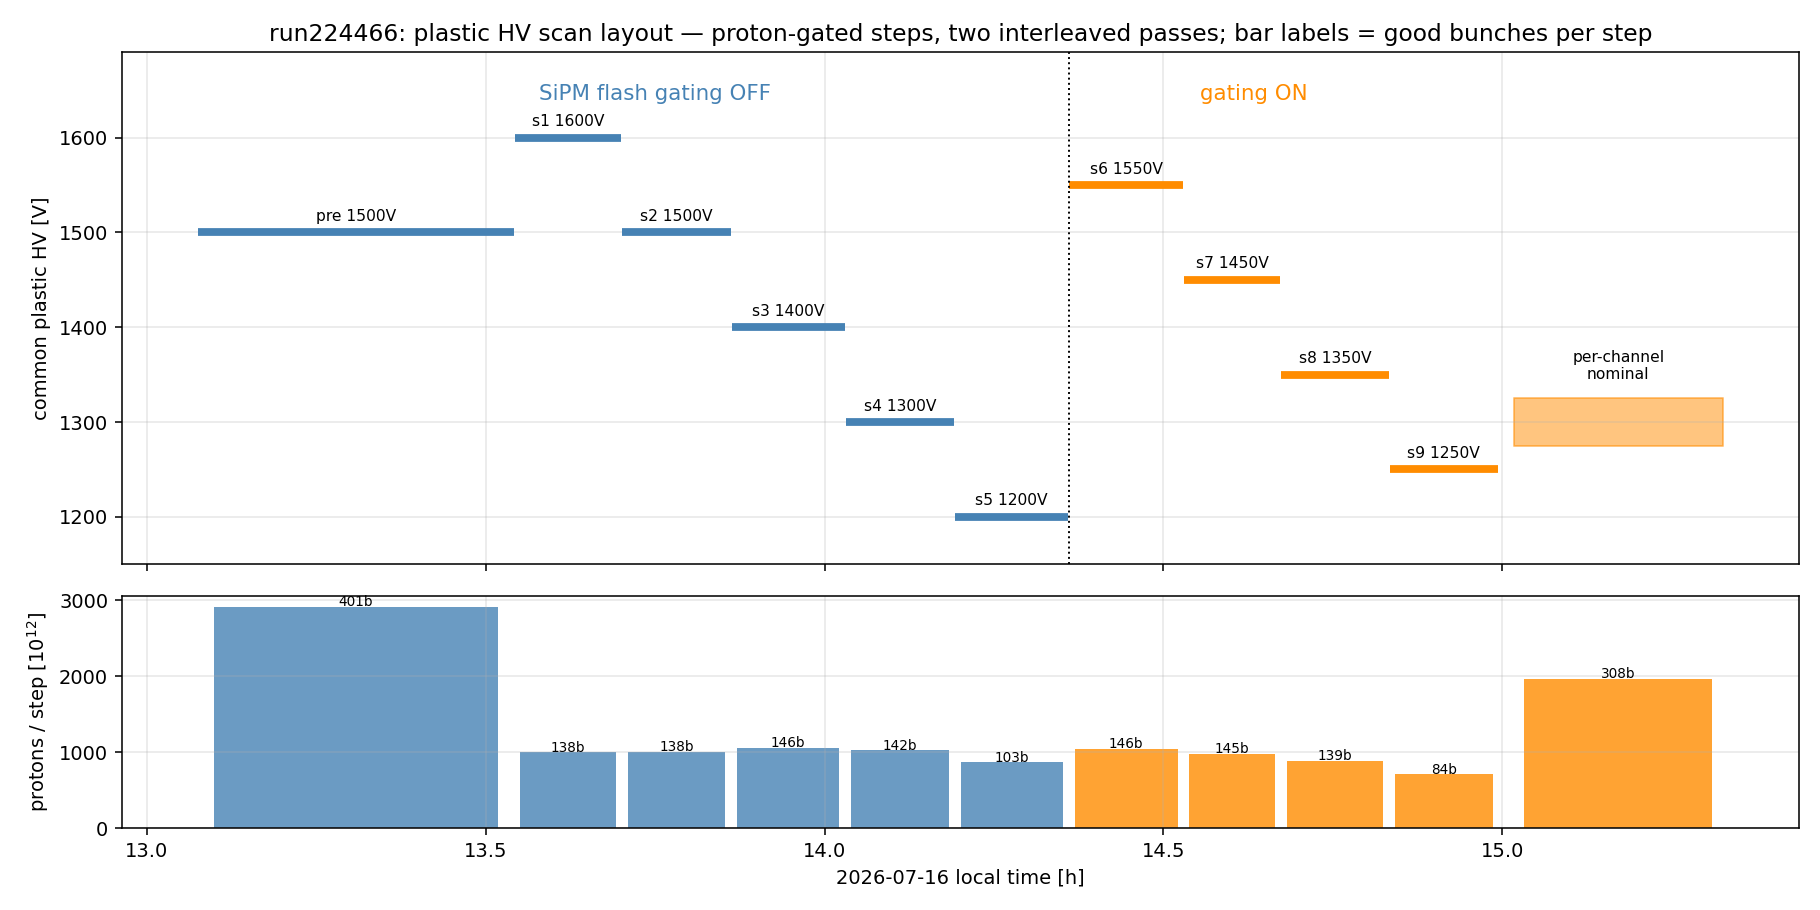
\includegraphics[width=0.95\textwidth]{12_hv_scan/scan_timeline.png}
  \caption{Scan layout: common plastic HV vs.\ wall-clock time (top; blue =
  flash-gating off, orange = on, dotted line = changeover) and delivered
  protons per step (bottom; labels = good bunches per step). The pre-scan
  \SI{1500}{\volt} stretch and the post-scan return to per-channel nominals
  provide two extra calibration windows.}
  \label{fig:timeline}
\end{figure}

\section{Gain observable: wall-tagged coincident spectra}
The \emph{inclusive} plastic hit spectrum is a poor gain observable: the
acquisition threshold sits well inside the steeply falling spectrum, so as the
gain rises more small pulses enter the sample and the median hardly moves (for
three PMTs it even decreases with voltage). Instead we use the wall-tagged
sample of the MIP analysis: plastic hits in a $\pm$8\,ns calibrated
coincidence with a same-arm wall channel (time offsets re-measured on this
run), sideband-subtracted with the $+20$ to $+120$\,ns window. The tag is
provided by the SiPM wall, whose response is independent of the plastic bias,
so the tagged plastic population is a fixed physical reference whose measured
amplitude tracks the PMT gain directly.

Figure~\ref{fig:spectra} shows the tagged spectra marching up with voltage at
fixed shape (log amplitude axis); Figure~\ref{fig:spectra_lin} shows the same
spectra as probability densities on a linear amplitude axis, with an arrow
marking each spectrum's median --- the single number per (PMT, voltage) that
the rest of the analysis uses. The median is chosen over a peak fit because
the tagged plastic spectrum has no sharp MIP peak (the plastic sits behind the
wall and the tag does not constrain path length in the plastic); once the
liquid-scintillator readout is available, a wall$\times$plastic$\times$LS
triple coincidence should isolate a true plastic MIP peak and allow an
absolute (rather than relative) energy calibration.
Figure~\ref{fig:gain} shows the median of the subtracted spectrum
versus the measured bias on log--log axes. Each PMT follows a single power law
$\mathrm{med}\propto V^{n}$: the two passes land on one curve (the gating state
does not disturb the gain measurement), the pre-scan \SI{1500}{\volt} window
reproduces the pass-1 \SI{1500}{\volt} step exactly, and the post-scan nominal
points fall on the fits. Fitted indices are listed in
Table~\ref{tab:equalize}; C-left, with the lowest index ($n=4.8$), visibly
flattens above $\sim$\SI{1500}{\volt}.

\begin{figure}[H]
  \centering
  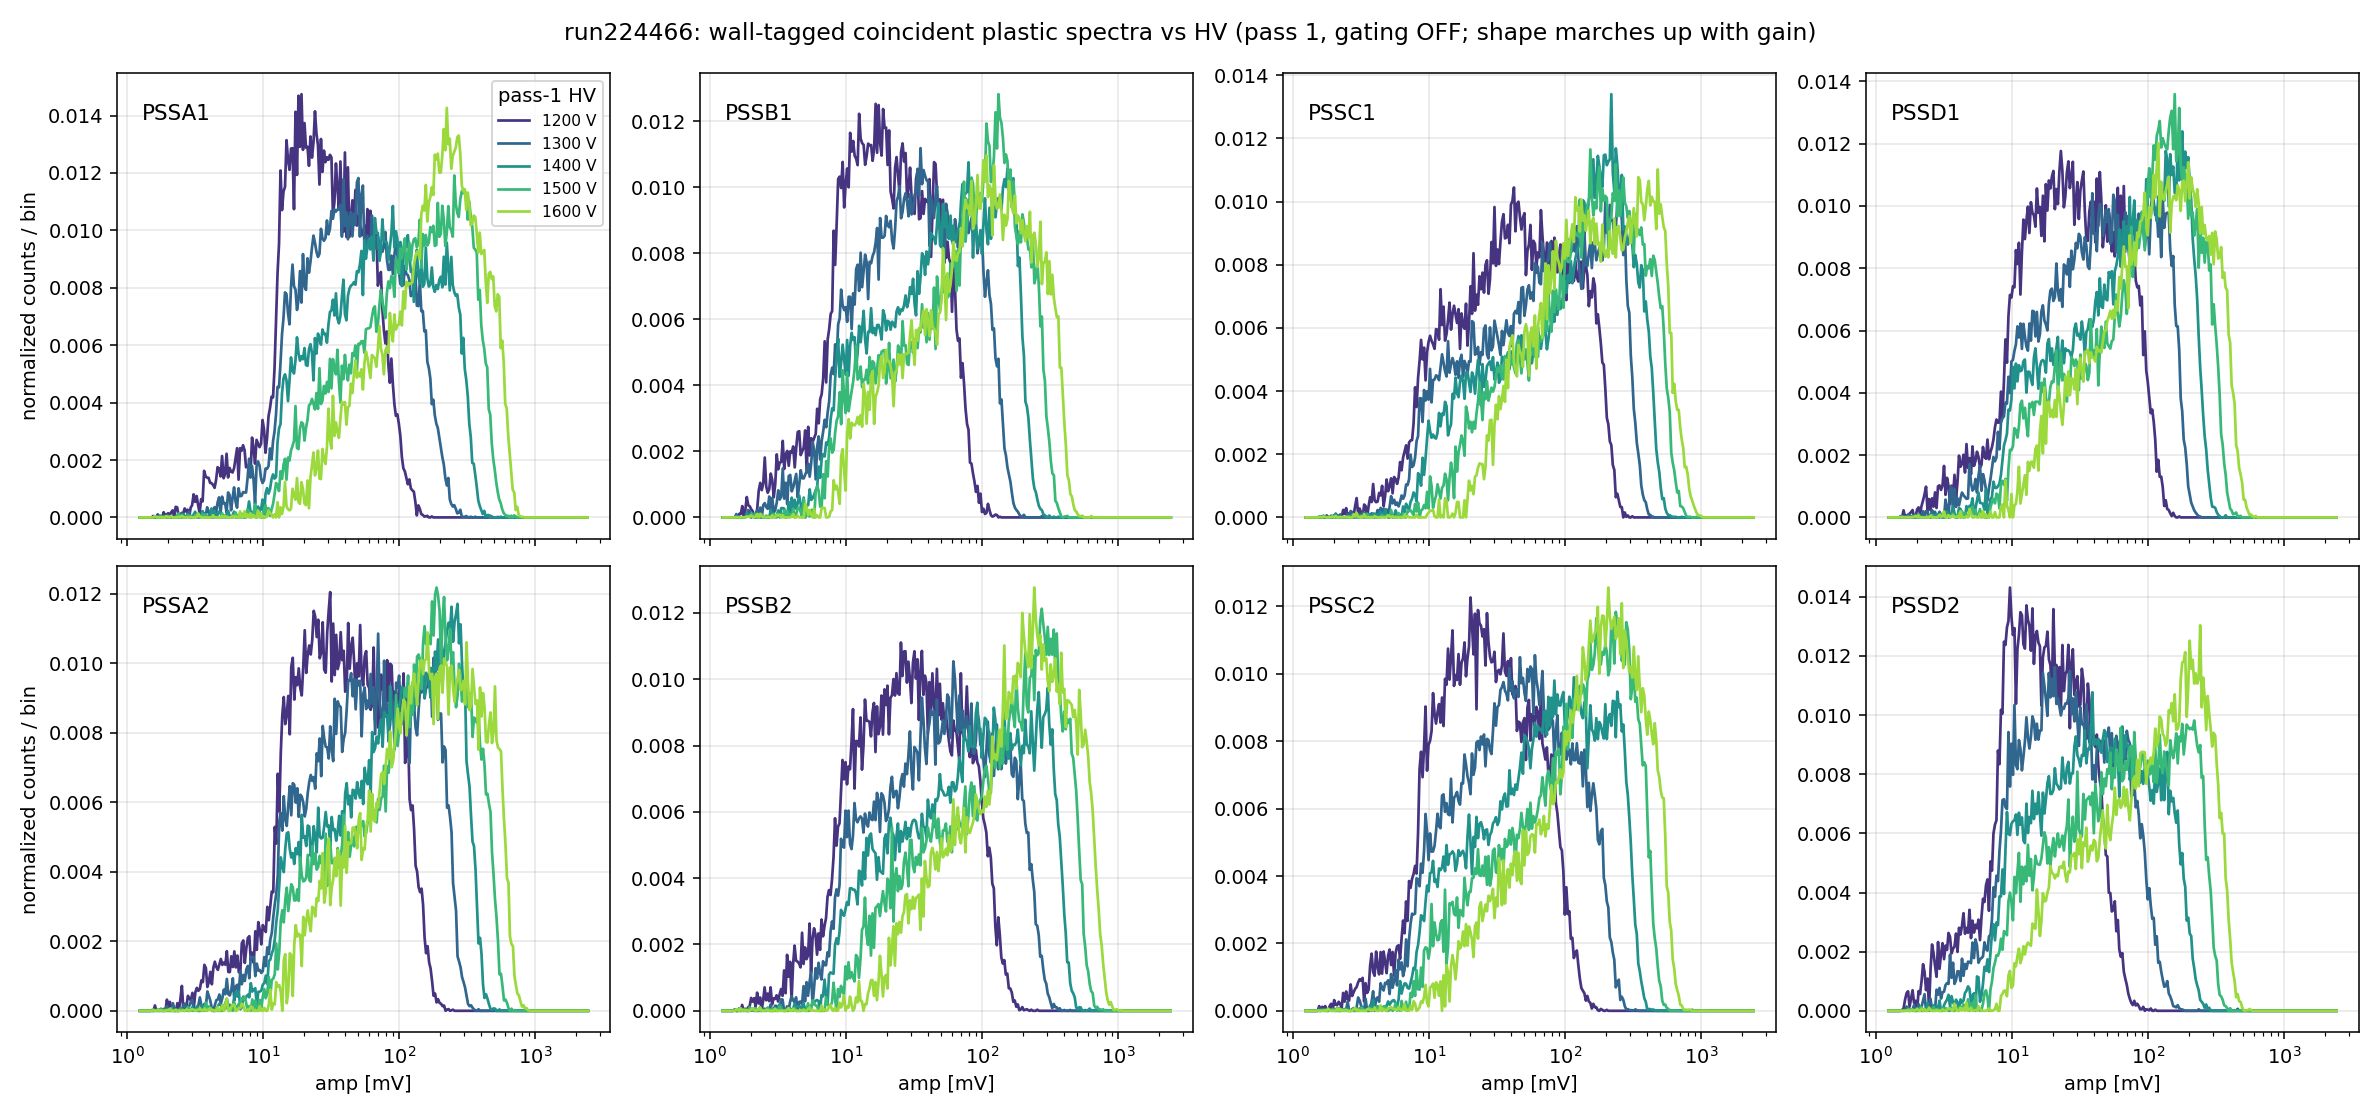
\includegraphics[width=\textwidth]{12_hv_scan/coinc_spectra.png}
  \caption{Wall-tagged, sideband-subtracted plastic amplitude spectra for the
  five pass-1 voltages (gating off), normalized to unit area. The population
  is fixed by the wall tag; the amplitude scale moves with the PMT gain.}
  \label{fig:spectra}
\end{figure}

\begin{figure}[H]
  \centering
  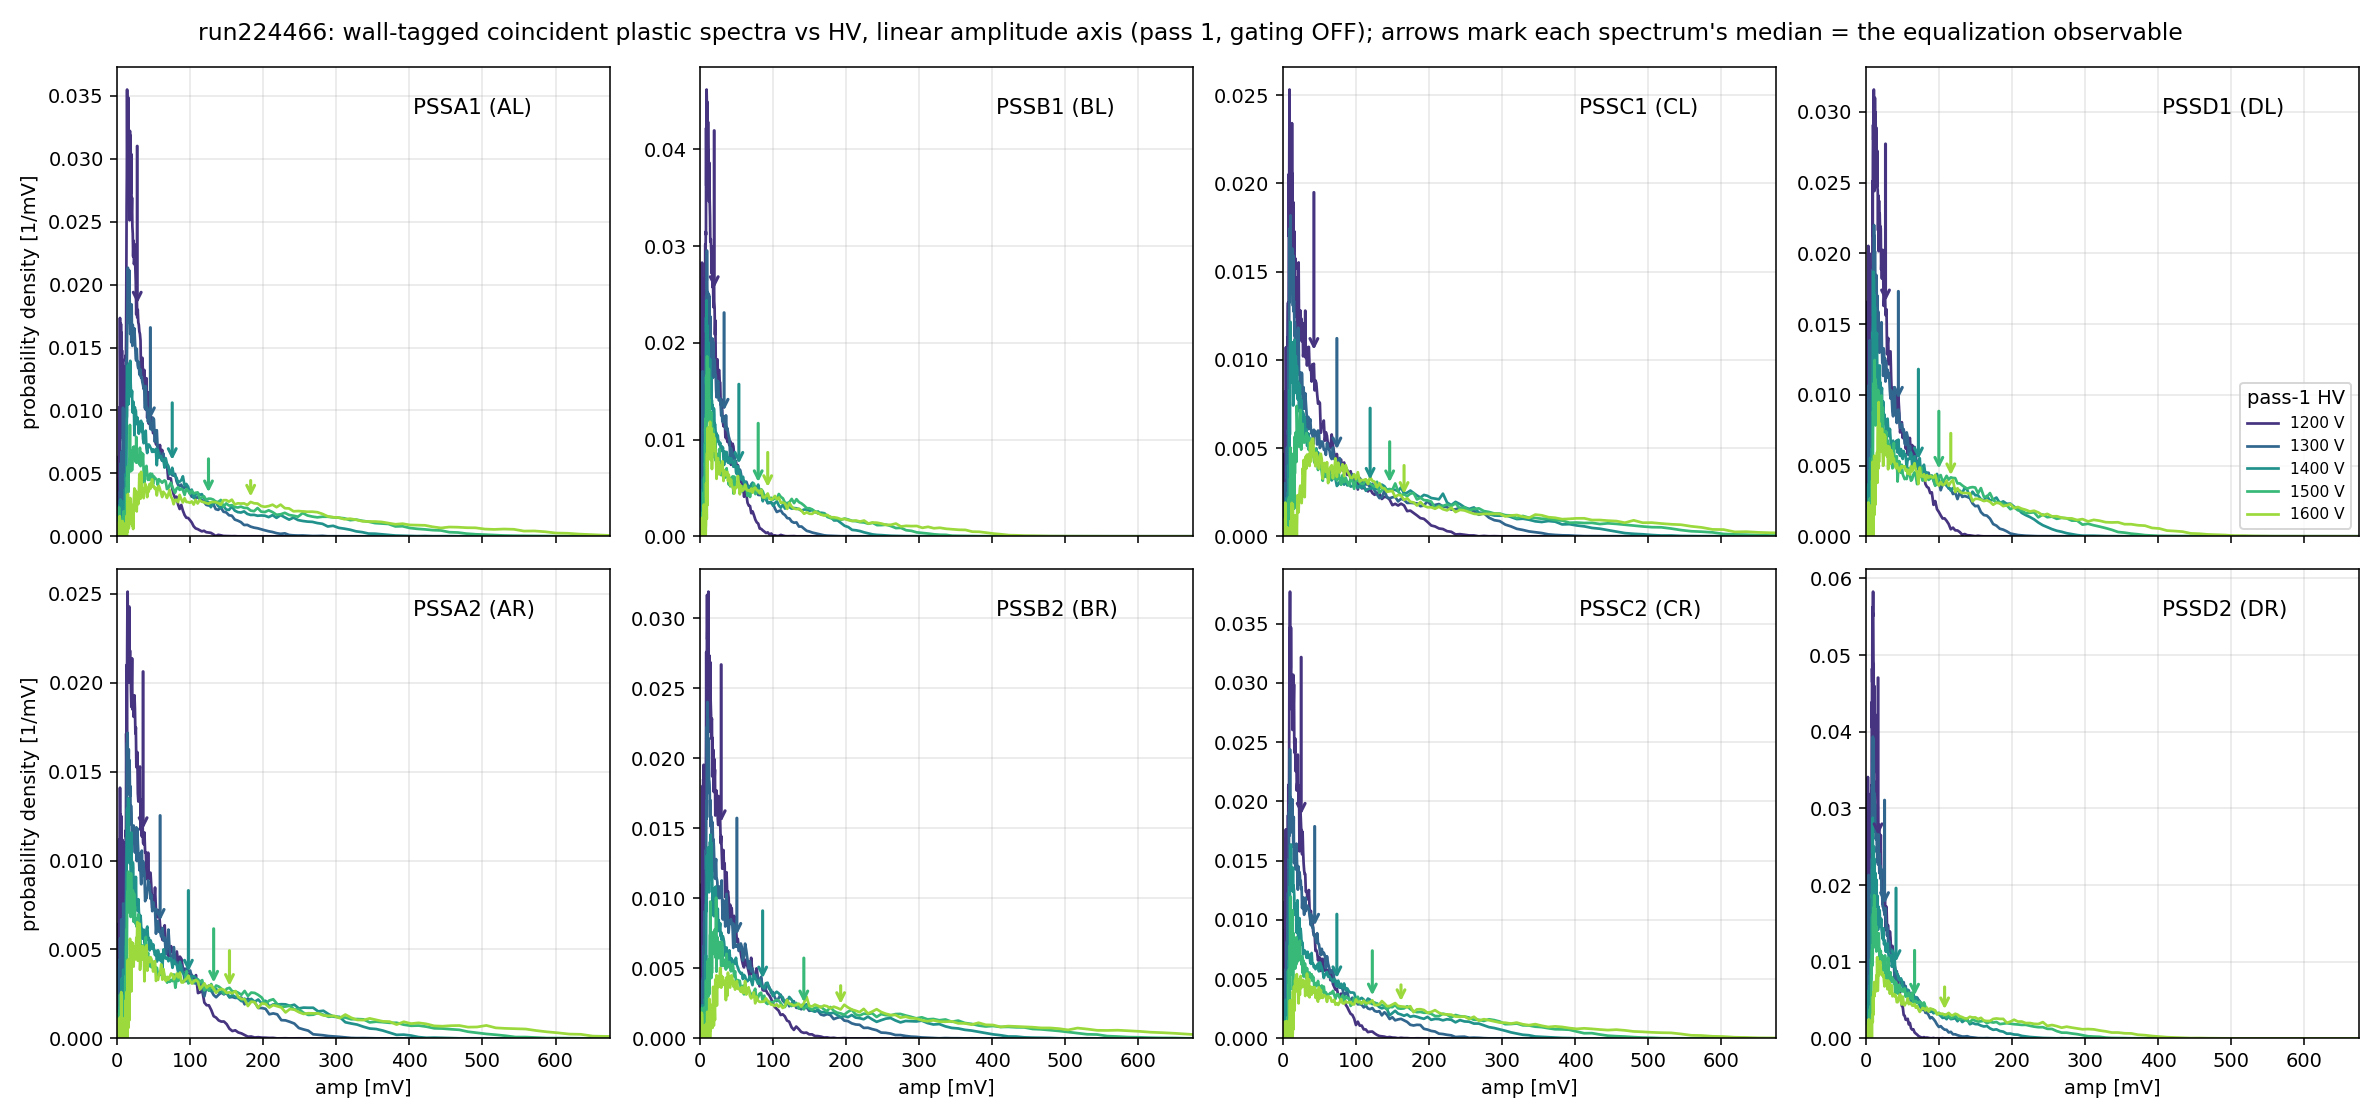
\includegraphics[width=\textwidth]{12_hv_scan/coinc_spectra_linear.png}
  \caption{The same tagged spectra as densities on a linear amplitude axis
  (pass 1), in mV (per-channel ADC$\to$mV factors, all
  $\approx\SI{0.0307}{\milli\volt}$/count). Arrows mark each spectrum's
  median, the equalization observable. The low-amplitude pile-up against the
  acquisition threshold, prominent at low voltage, is why the
  \emph{inclusive} median is not a usable gain proxy.}
  \label{fig:spectra_lin}
\end{figure}

\begin{figure}[H]
  \centering
  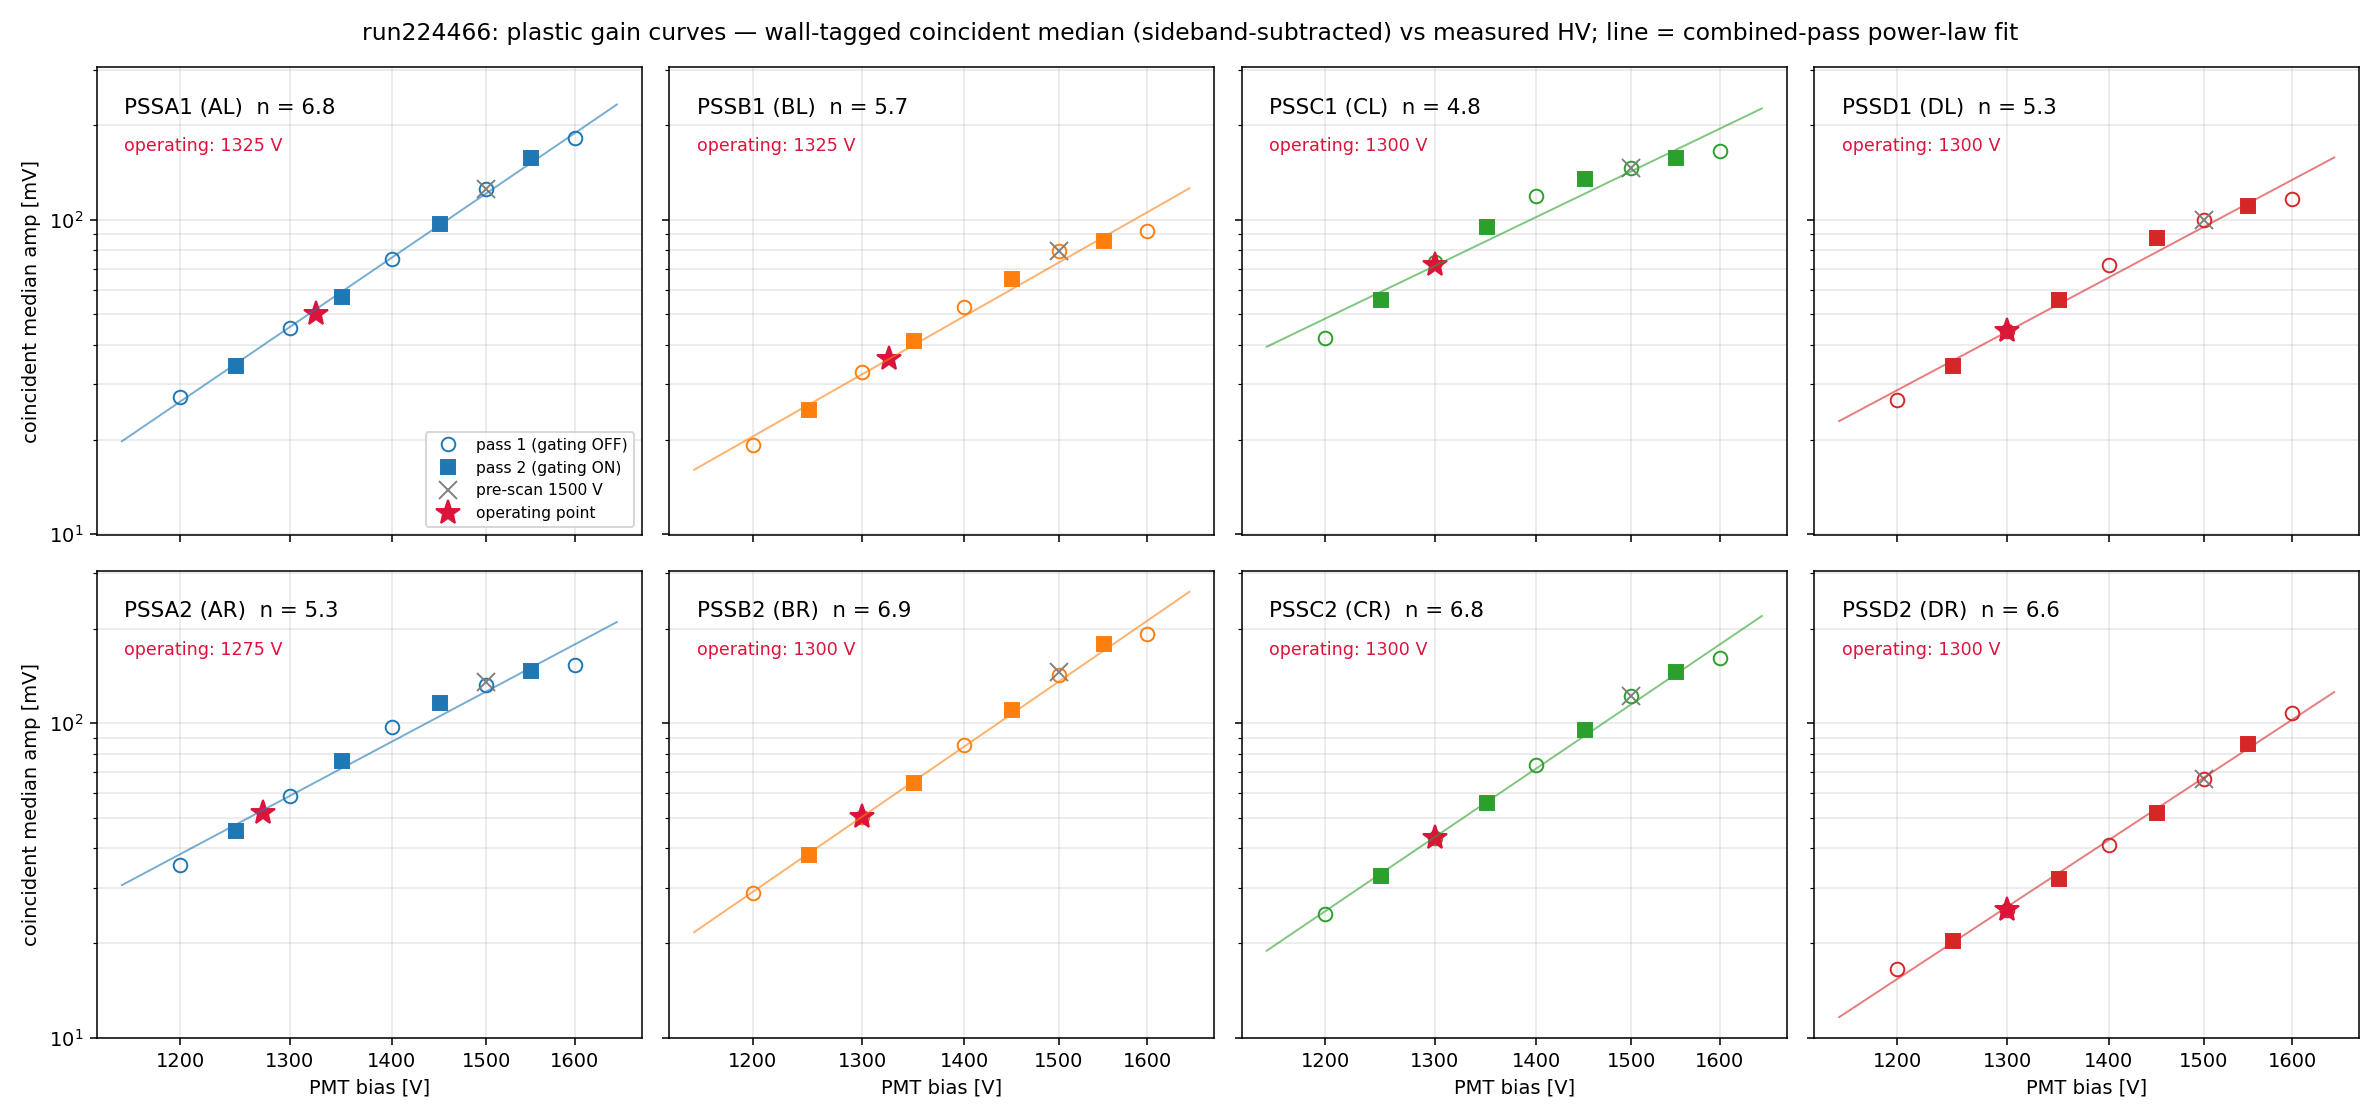
\includegraphics[width=\textwidth]{12_hv_scan/gain_curves.png}
  \caption{Coincident median amplitude vs.\ measured bias (log--log), per PMT;
  the operating voltage is noted in each panel.
  Open circles: pass 1 (gating off); filled squares: pass 2 (gating on);
  gray cross: pre-scan \SI{1500}{\volt} window; star: post-scan operating
  point. Lines: combined-pass power-law fits (indices in
  Table~\ref{tab:equalize}).}
  \label{fig:gain}
\end{figure}

\section{HV equalization}
At the current operating voltages the tagged-median response spans a factor
$2.8$ (C-left highest, D-right lowest). Table~\ref{tab:equalize} gives, per
PMT, the voltage that brings its response to a common target using that PMT's
own fitted index; Fig.~\ref{fig:equalize} shows the construction --- each PMT
slides along its own gain curve to the target line. These measured exponents
supersede the $G\propto V^{7}$ assumption used for the provisional
suggestions in the run-224404 report.

\paragraph{Choice of the absolute target.} The target is simply the
\emph{geometric mean of the eight current responses} (1461~ADC $\approx$
\SI{45}{\milli\volt}) --- an ``equalize around where we already operate''
choice, not one derived from an independent requirement. It is not
rate-informed: the rate curves (Fig.~\ref{fig:rates}) show no plateau, so
there is no counting-efficiency optimum to aim at, and the plastic threshold
in the n\_TOF PSA is an analysis quantity rather than a hardware trigger
level. The geometric mean minimizes the collective HV movement (the
suggested steps stay within $-120$/$+117$\,V of present values, inside the
scanned, validated range) and keeps the fleet's occupancies and pile-up
behavior close to the operating point already characterized. Setting the
absolute scale to something physically motivated --- e.g.\ a plastic MIP at a
chosen mV value --- is deferred until the liquid-scintillator readout allows a
true plastic MIP calibration; the power laws measured here then convert any
such target into voltages directly.

\begin{figure}[H]
  \centering
  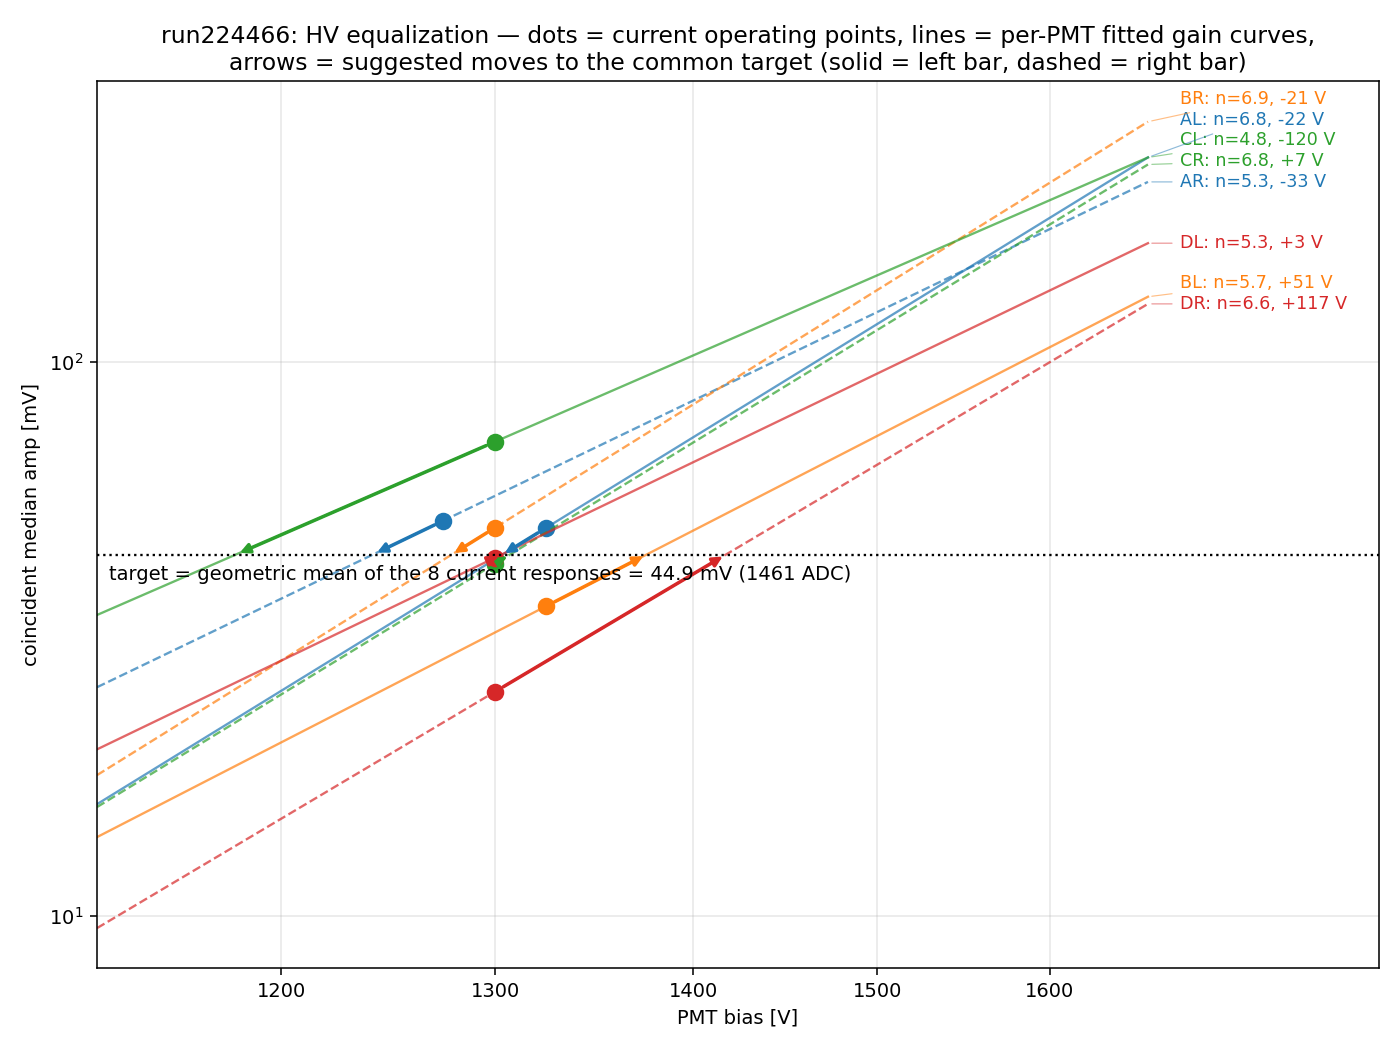
\includegraphics[width=0.8\textwidth]{12_hv_scan/equalization.png}
  \caption{The equalization construction. Dots: current operating points
  (tagged median from the post-scan window). Lines: per-PMT power laws
  $G(V)=\mathrm{med}_\mathrm{now}(V/V_\mathrm{now})^{n}$. Arrows: suggested
  moves to the common target (dotted line), the geometric mean of the eight
  current responses. Right-edge labels give each PMT's index and suggested
  $\Delta V$.}
  \label{fig:equalize}
\end{figure}

\begin{table}[H]
  \centering
  \caption{Fitted gain indices and voltage equalization to the fleet
  geometric-mean tagged median (1461 ADC = \SI{44.9}{\milli\volt}).
  $V_\mathrm{now}$ are the operating voltages after the scan; medians from
  the post-scan window (per-channel ADC$\to$mV from the DAQ full scale,
  $\approx\SI{0.0307}{\milli\volt}$/count).}
  \label{tab:equalize}
  \begin{tabular}{lS[table-format=4.0]S[table-format=4.0]S[table-format=2.1]S[table-format=1.2]S[table-format=4.0]S[table-format=+3.0]}
    \toprule
    PMT & {$V_\mathrm{now}$ [V]} & {median [ADC]} & {median [mV]} & {$n$} & {$V_\mathrm{sugg}$ [V]} & {$\Delta V$ [V]} \\
    \midrule
    A-L (PSSA1) & 1325 & 1637 & 50.2 & 6.83 & 1303 & -22 \\
    A-R (PSSA2) & 1275 & 1679 & 51.7 & 5.34 & 1242 & -33 \\
    B-L (PSSB1) & 1325 & 1178 & 36.2 & 5.71 & 1376 & +51 \\
    B-R (PSSB2) & 1300 & 1637 & 50.2 & 6.90 & 1279 & -21 \\
    C-L (PSSC1) & 1300 & 2334 & 71.8 & 4.83 & 1180 & -120 \\
    C-R (PSSC2) & 1300 & 1406 & 43.2 & 6.79 & 1307 & +7 \\
    D-L (PSSD1) & 1300 & 1442 & 44.3 & 5.35 & 1303 & +3 \\
    D-R (PSSD2) & 1300 &  826 & 25.4 & 6.59 & 1417 & +117 \\
    \bottomrule
  \end{tabular}
\end{table}

\section{Stability of the wall MIP calibration}
The scan is also a controlled test of the MIP method itself: if the
wall--plastic coincidence selection biased the wall amplitude, the wall MIP
peak would move as the plastic gain --- and with it the tag rate and its
pulse-height mix --- changes by a factor of a few. It does not.
Figure~\ref{fig:stability} shows the channel-summed, sideband-subtracted wall
MIP peak per arm and per step, normalized to its scan mean: all four arms stay
within one amplitude bin ($\pm2.6\%$) from \SI{1200}{\volt} to
\SI{1600}{\volt} and across the gating boundary. The wall MIP calibration
(channel-summed on this run: A $\approx$ 817 ADC = \SI{25.0}{\milli\volt},
B $\approx$ 1191 = \SI{36.4}{\milli\volt}, C $\approx$ 1175 =
\SI{35.9}{\milli\volt}, D $\approx$ 1162 = \SI{35.5}{\milli\volt}) can
therefore be used independently of the plastic operating point, including
after the equalization of Table~\ref{tab:equalize}.

\begin{figure}[H]
  \centering
  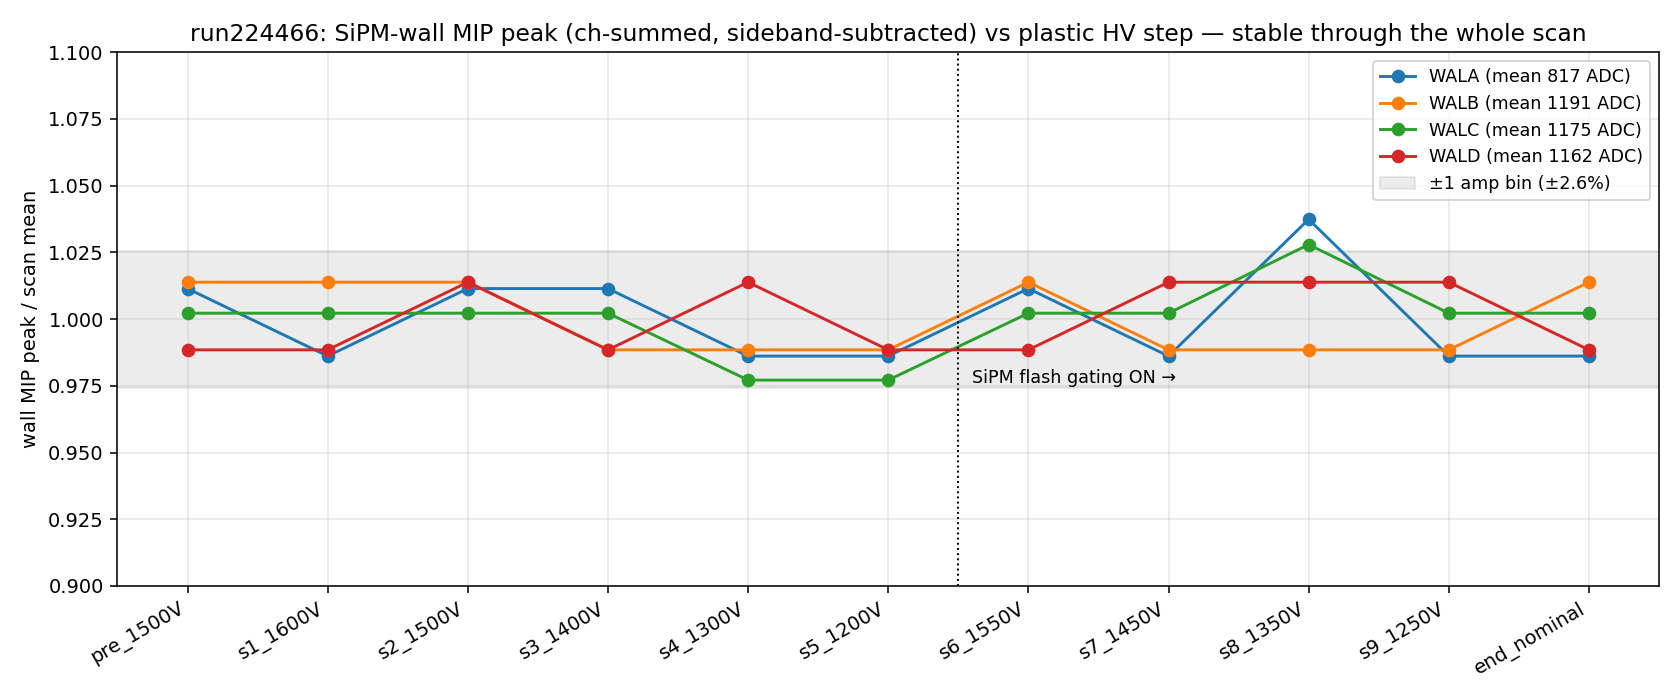
\includegraphics[width=0.85\textwidth]{12_hv_scan/wall_mip_stability.png}
  \caption{Wall MIP peak (channel-summed, sideband-subtracted) per arm vs.\
  scan step, normalized to the scan mean. Gray band: one histogram bin
  ($\pm2.6\%$). Dotted line: SiPM flash-gating turned on.}
  \label{fig:stability}
\end{figure}

\section{Rates and the flash-gating check}
The late-time plastic hit rate per proton rises monotonically with voltage
with no plateau up to \SI{1600}{\volt}
(Fig.~\ref{fig:rates}) --- the threshold sits inside the physical spectrum at
every voltage, so counting-plateau HV setting is not applicable here; the
equalization above is the amplitude-based alternative. The rates are
unaffected by the gating state (pass-1 and pass-2 points fall on one curve).
In the $\gamma$-flash window itself, wall occupancy drops by only
$\sim$4--6\% with gating on --- much weaker than a blanking of the SiPM
readout during the flash would suggest; what the M6.C ``SiPM enable'' pulse
actually diverts should be checked with the hardware experts.

\begin{figure}[H]
  \centering
  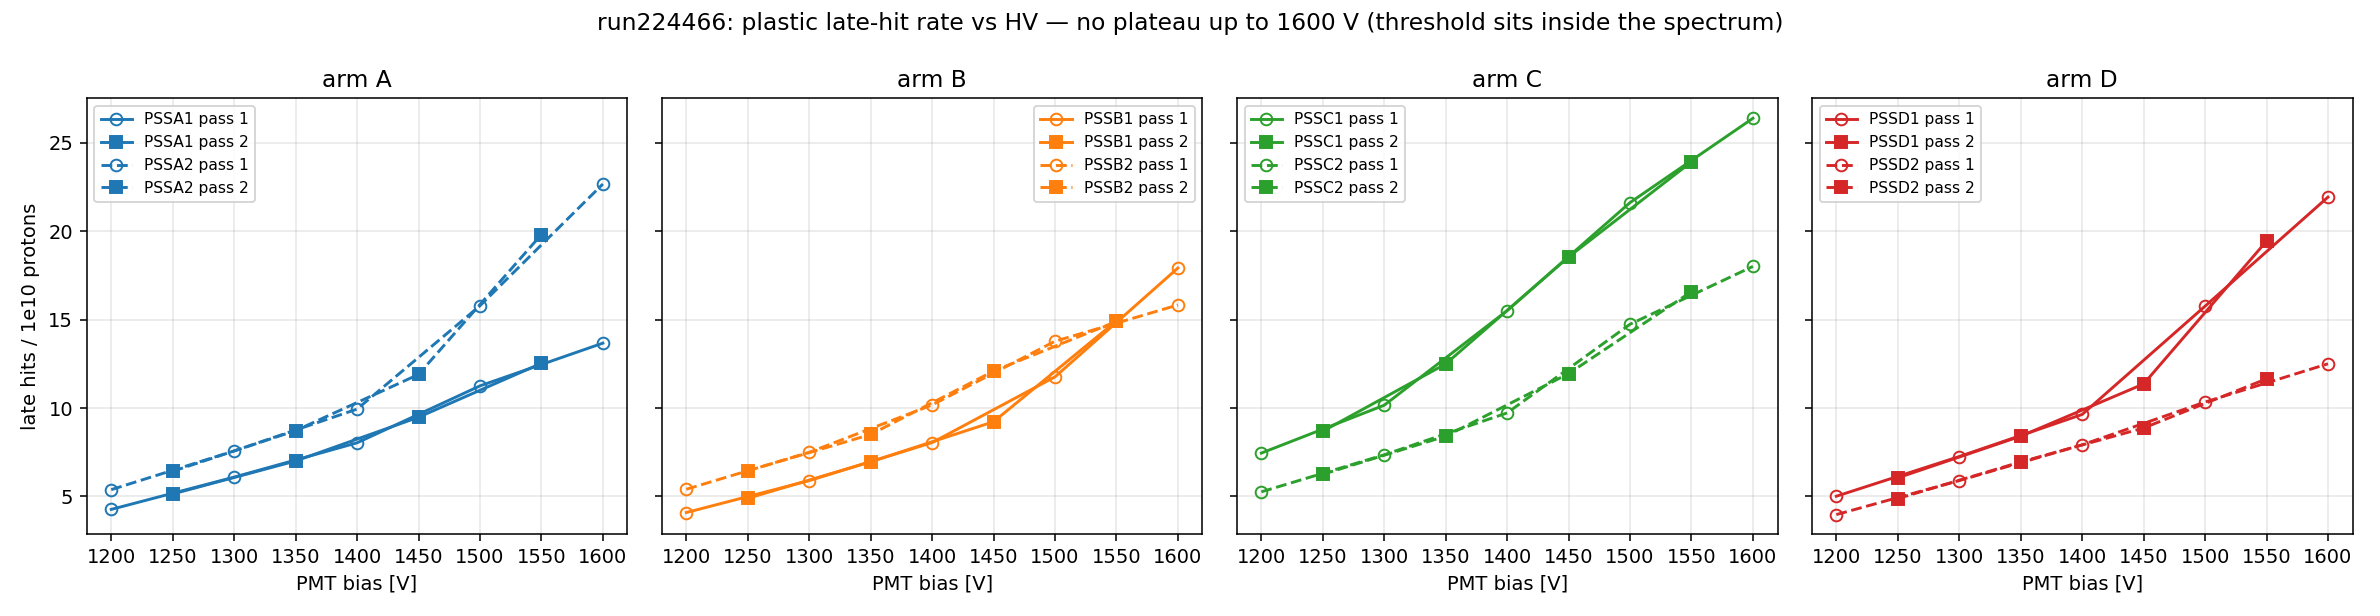
\includegraphics[width=\textwidth]{12_hv_scan/rate_curves.png}
  \caption{Plastic late-time hit rate per $10^{10}$ protons vs.\ bias. Solid:
  left bars; dashed: right bars; open/filled markers: pass 1/2.}
  \label{fig:rates}
\end{figure}

\section{A first plastic trigger threshold}
If the plastics are to participate in a trigger, the natural question is how
low the discriminator can sit. There is no signal/noise valley to aim for:
the tagged spectra rise monotonically toward the acquisition cutoff
($\sim$\SIrange{1.5}{2}{\milli\volt}, the n\_TOF PSA threshold of
$\sim$50~ADC counts — nothing below it is recorded, so lower settings are
unexplored territory). The choice is therefore efficiency-driven.
Figure~\ref{fig:threshold} scans a \emph{common} threshold on the
post-equalization amplitude scale (each PMT's measured spectrum scaled by its
equalization factor, so one value serves all eight): the wall-tagged
population — our best proxy for real particles — is kept at $\geq$99\% on
every PMT down to \SI{4.2}{\milli\volt} and $\geq$95\% down to
\SI{6.3}{\milli\volt}, while the accepted late-time hit rate falls by
$\sim$15\% (25\%) relative to threshold-free.

Unconstrained, the natural choice would be \SIrange{4}{5}{\milli\volt}
(digitizer-equivalent, post-equalization) — safely above the acquisition
cutoff and the near-threshold pile-up, $\geq$99\% efficient for the tagged
population everywhere. \textbf{In practice the discriminator hardware has a
\SI{10}{\milli\volt} floor}, where the worst PMT keeps 86\% of the tagged
population (range 86--97\% over the eight, at the equalized gains). Two ways
forward: (a) accept the 10\,mV floor at the present gains — the current plan
until a true plastic MIP calibration exists; or (b) raise all gains by a
common factor with the per-PMT power laws so that \SI{10}{\milli\volt} sits
at today's 99\% (95\%) point: gain $\times2.35$ ($\times1.59$), i.e.\
equalized voltages moving to 1408--1614\,V (1298--1520\,V) — only the
$\times2.35$ value for D-R exceeds the validated scan range. Higher gain
also multiplies the accepted rate and moves the tagged median to
$\sim$\SI{105}{\milli\volt}; pile-up and dynamic range should be rechecked
before adopting it. Caveats: these are digitizer-equivalent mV (map to
hardware discriminator units before setting); the rate axis is the late-TOF
in-spill sample (relative, not an absolute trigger rate — the $\gamma$-flash
region adds its own, much larger, instantaneous rate). These numbers are
exported to the DAQ repo (\path{calibrations/pss_trigger/}).

\begin{figure}[H]
  \centering
  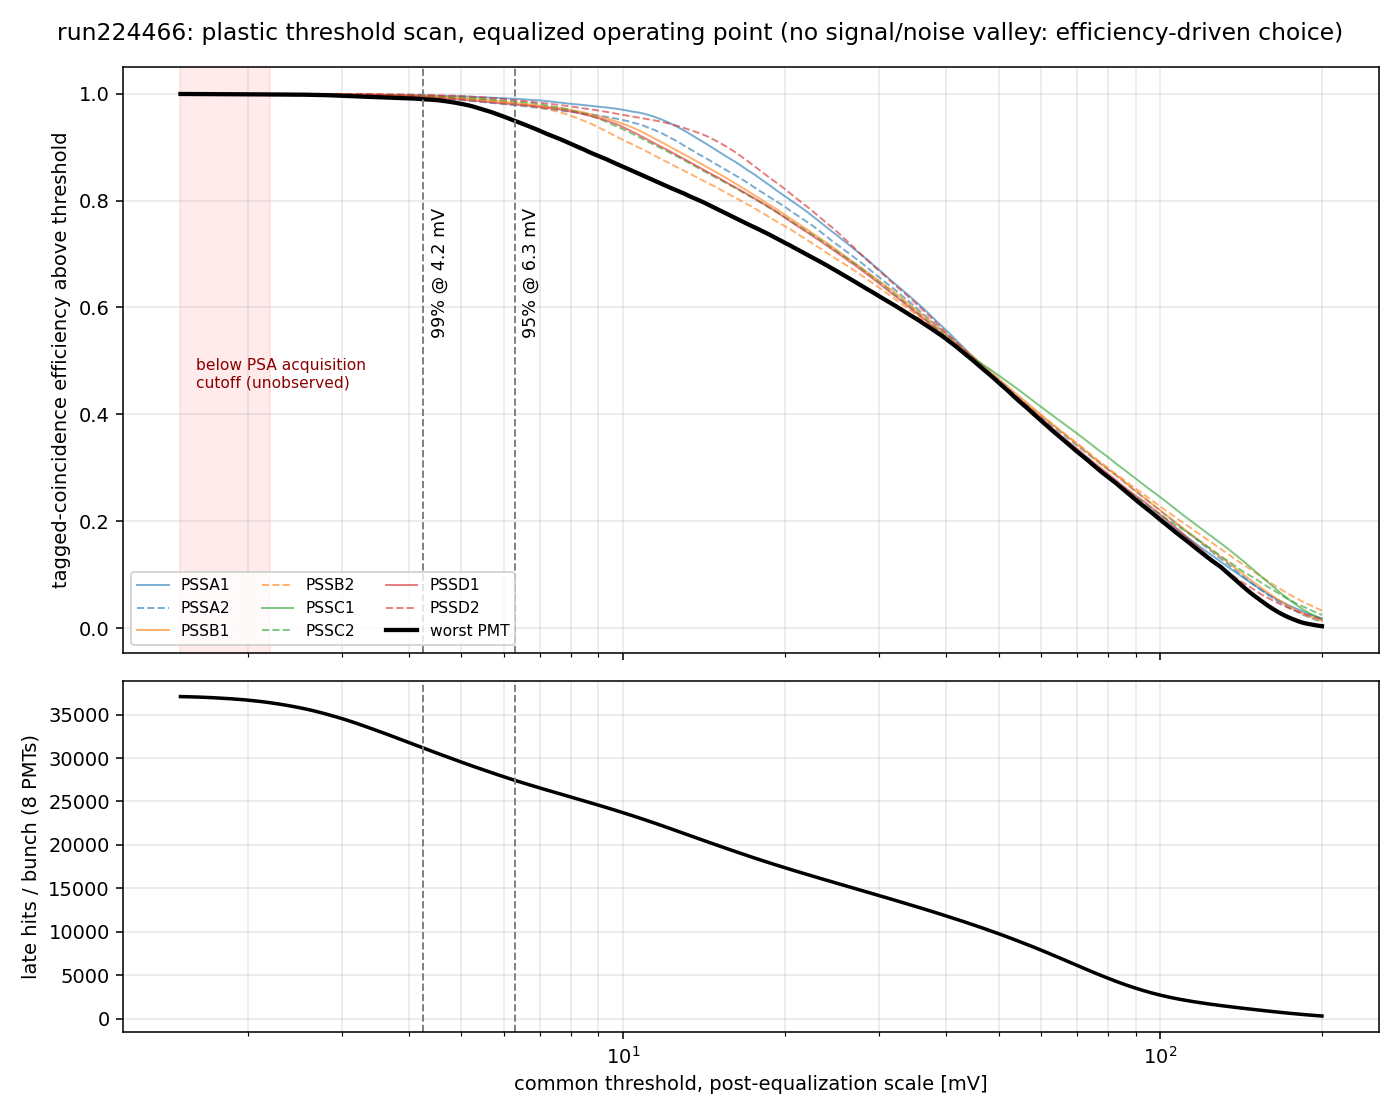
\includegraphics[width=0.85\textwidth]{12_hv_scan/threshold_scan.png}
  \caption{Common-threshold scan at the equalized operating point. Top:
  wall-tagged (sideband-subtracted) efficiency above threshold per PMT (thin,
  solid = left / dashed = right bars) and the worst PMT (bold); dashed
  verticals: 99\% and 95\% points of the worst PMT. Red band: below the PSA
  acquisition cutoff (unobserved). Bottom: total accepted late-time hits per
  bunch (8 PMTs, relative scale).}
  \label{fig:threshold}
\end{figure}

\section*{Reproducibility}
HV log and scan handoff: \path{~/beam_july/scint_hv_scan/2026-07-16_13-32-34_plastic_scan_1/}
(pulled from the DAQ machine). Analysis:
\texttt{mx\_july\_beam\_qa/12\_plastic\_hv\_scan.py} (accumulation, cache
\texttt{cache/12\_hvscan\_run224466.npz}) and \texttt{12b\_hv\_scan\_plots.py}
(figures and Table~\ref{tab:equalize}), running on the binary hit cache of the
fast read pass (\texttt{fastread/}, \texttt{hitcache.py}; full-run turnaround
$\sim$3 minutes).

\end{document}
